%% Figure C17. Where the best squares of PHerc. 0826 sit relative to each other: the part of one axial slice
%% of the raw scan around the squares (since 2026-09-30 without the whole slice, the scroll's outline or any
%% height), with the published umbilicus, the crossings of the delivered sheets of the marked seeds, and the
%% centre of each best square. The rasters and every coordinate, label
%% and number of the overlay are written by tools/c-f17-where-squares.py from the rows of
%% ../evidence/figures/c-f17-where-squares.csv; the body is c-f17-where-squares-body.tex. Nothing but the
%% styles is typed here. NO INK.
\documentclass[border=1pt]{standalone}
%% THIS FILE IS SHARED. Its one source is results/figpreamble.tex and the copy in each work's
%% src/tools is taken from it, because a published folder has to stand on its own and cannot
%% follow a link out of itself. tools/check_figpreamble.py refuses a copy that has drifted.
%%
%% It is one file because it was two, and they drifted: the panel title correction of
%% 2026-09-22T06:44Z was made in one work's copy and never reached the other, so that work drew
%% both panel titles at the axis origin, inside the plot and over the first bar, until
%% 2026-09-22T14:33Z. One source and a check is what stops that happening twice.

%% figpreamble.tex: what every figure of this work loads, and the one filter they all use.
%%
%% Every figure is a standalone pgfplots document that reads its numbers with pgfplotstable from
%% the CSV its own data script wrote under evidence/figures/. No number is typed in a figure
%% source. That is not a style: it is what makes the picture and the table of plotted numbers
%% unable to disagree, because they are the same file read twice.
%%
%% The CSVs written by tools/figlib.py open with one comment line, so every table is read with
%% skip first n=1, and they carry no comma inside a cell, so col sep=comma is exact.
\usepackage{pgfplots}
\usepackage{pgfplotstable}
\pgfplotsset{compat=1.18}
\usepgfplotslibrary{groupplots}

\pgfplotstableset{col sep=comma, skip first n=1, trim cells}

%% One CSV per figure, and no filtering in the figure source.
%%
%% The plotted tables are wide: one row per position on the abscissa, one column per series.
%% That is not a taste, it is what works. pgfplotstable parses every cell of a column an
%% \addplot names, and its read time row filter does not see column values, so a long table with
%% one row per series cannot be split inside the figure: the rows of the other series are parsed
%% too. The first render of figure S2 failed on exactly that, on the cell "not measurable", and
%% the tables were rewritten wide. A series with no value at a position carries nan, which
%% pgfplots drops with its default unbounded coords setting, and never a zero; the words the
%% study used sit in the status column beside the number.

%% One neutral set of marks and fills, light background, no colour carrying meaning on its own:
%% every series is also told apart by its mark, because a reader printing in grey is still a
%% reader.
\pgfplotsset{
  sa base/.style={
    width=82mm, height=58mm,
    tick align=outside, tick pos=left,
    grid=major, grid style={gray!25, very thin},
    axis line style={gray!60},
    label style={font=\small}, tick label style={font=\footnotesize},
    legend style={font=\footnotesize, draw=gray!50, fill=white, fill opacity=0.9,
                  text opacity=1, cells={anchor=west}},
    %% The title sits ABOVE the panel and not on it: with `above` alone it landed on the
    %% plot area and over the tick labels of the panel beside it, seen 2026-09-22T06:44Z.
    every axis title/.style={font=\small, at={(0.5,1)}, anchor=south, yshift=2.5mm},
  },
  %% A legend BELOW the panel, outside the plot area entirely, in one row.
  %%
  %% Written 2026-09-22 on the director's rejection of figure S1. `sa base` gives the legend
  %% `fill opacity=0.9`, so a legend placed inside does not hide what is under it, it GHOSTS it:
  %% on S1 the legend sat over the seed40 pair and its «200 times» label showed through the box
  %% as pale grey text, which is worse than hiding it, because a reader sees something is there
  %% and cannot read it. The remedy is not a better corner. A legend inside the plot area has to
  %% be re placed by hand every time the data moves, and nobody checks. Outside, it cannot
  %% collide with anything at any data value.
  %%
  %% The negative y in `at` is in axis fractions, so it follows `height` and does not have to be
  %% retuned. 0.32 clears rotated tick labels at \tiny; a panel with longer ones passes its own.
  sa legend below/.style={
    legend style={at={(0.5,-0.32)}, anchor=north, legend columns=-1,
                  font=\footnotesize, draw=gray!50, fill=white, fill opacity=1,
                  text opacity=1, cells={anchor=west},
                  /tikz/every even column/.append style={column sep=4mm}},
  },
  sa bars/.style={
    sa base, ybar, bar width=4pt, enlarge x limits=0.08,
  },
  sa stacked/.style={
    sa base, ybar stacked, bar width=14pt, enlarge x limits=0.28,
  },
}
\definecolor{sablue}{RGB}{31,78,121}
\definecolor{saorange}{RGB}{191,98,4}
\definecolor{sagrey}{RGB}{110,110,110}
\definecolor{sagreen}{RGB}{31,110,70}

%% ---- Addition of 2026-09-28T18:30Z (coordinator, director's note of 18:29:38Z, owner's word) ----
%% One visual language across S, A, the umbilicus and the PHerc. 0826 article: IEEE serif type and
%% one colour blind safe palette, the Okabe and Ito set (Okabe M., Ito K., Color Universal Design,
%% 2002, the eight colours of its table). The four names above keep their names and take Okabe Ito
%% values, so every figure that already uses them follows. Colours carry a ROLE, the umbilicus
%% work's rule: our result blue, the reference or the published label orange, an outcome we do not
%% want vermillion; a second series of ours sky blue, a third bluish green; neutral grey. The same
%% values, under the same role names, are in results/figstyle.py for the rasters and matplotlib.
\usepackage{mathptmx}
\definecolor{sablue}{RGB}{0,114,178}
\definecolor{saorange}{RGB}{230,159,0}
\definecolor{sagrey}{RGB}{110,110,110}
\definecolor{sagreen}{RGB}{0,158,115}
\definecolor{sasky}{RGB}{86,180,233}
\definecolor{savermillion}{RGB}{213,94,0}
\definecolor{sapurple}{RGB}{204,121,167}
\definecolor{sayellow}{RGB}{240,228,66}
\colorlet{saours}{sablue}
\colorlet{saref}{saorange}
\colorlet{sabad}{savermillion}
\pgfplotscreateplotcyclelist{sa roles}{
  {sablue, mark=*}, {saorange, mark=square*}, {sasky, mark=triangle*},
  {sagreen, mark=diamond*}, {savermillion, mark=pentagon*}, {sapurple, mark=o}, {sagrey, mark=x}}
\pgfplotsset{sa base/.append style={cycle list name=sa roles, axis x line*=bottom, axis y line*=left}}

\usetikzlibrary{shapes.geometric}
\begin{document}
\newcommand{\ctkey}{\tikz[baseline=-0.6ex]\node[ct]{};\,}
\newcommand{\hfkey}{\tikz[baseline=-0.6ex]\node[hf]{};\,}
\newcommand{\lgkey}{\tikz[baseline=-0.6ex]\node[lg]{};\,}
\newcommand{\umbkey}{\tikz[baseline=-0.6ex]\node[umb]{};\,}
\newcommand{\sheetkey}{\tikz[baseline=-0.6ex]\draw[sagreen, line width=0.8pt] (0,0) -- (0.3,0);\,}
\begin{tikzpicture}[
  ct/.style={draw=black, fill=sasky, rectangle, minimum size=3.6pt, inner sep=0pt, line width=0.3pt},
  hf/.style={draw=saorange, fill=none, rectangle, minimum size=5pt, inner sep=0pt, line width=0.8pt},
  lg/.style={draw=black, fill=saorange, diamond, minimum size=5.4pt, inner sep=0pt, line width=0.3pt},
  umb/.style={draw=black, fill=sayellow, circle, minimum size=4.4pt, inner sep=0pt, line width=0.4pt},
  lab/.style={font=\scriptsize, align=left, fill=white, fill opacity=0.88, text opacity=1, inner sep=1.2pt,
              rounded corners=0.8pt},
  key/.style={font=\scriptsize, align=left, fill=white, fill opacity=0.88, text opacity=1, inner sep=1.5pt},
  note/.style={font=\scriptsize\itshape, fill=white, fill opacity=0.88, text opacity=1, inner sep=1.2pt},
  lead/.style={draw=white, line width=0.35pt},
  zoombox/.style={draw=white, line width=0.5pt},
  panlab/.style={font=\footnotesize, text=white, fill=black, fill opacity=0.6, text opacity=1, inner sep=1.2pt},
  bar/.style={draw=white, line width=1.4pt},
  barlab/.style={font=\scriptsize, text=white, fill=black, fill opacity=0.55, text opacity=1, inner sep=1pt}]
% Generated by src/tools/c-f17-where-squares.py from evidence/figures/c-f17-where-squares.csv. Do not edit.
\node[anchor=north west, inner sep=0] at (0,0.0000) {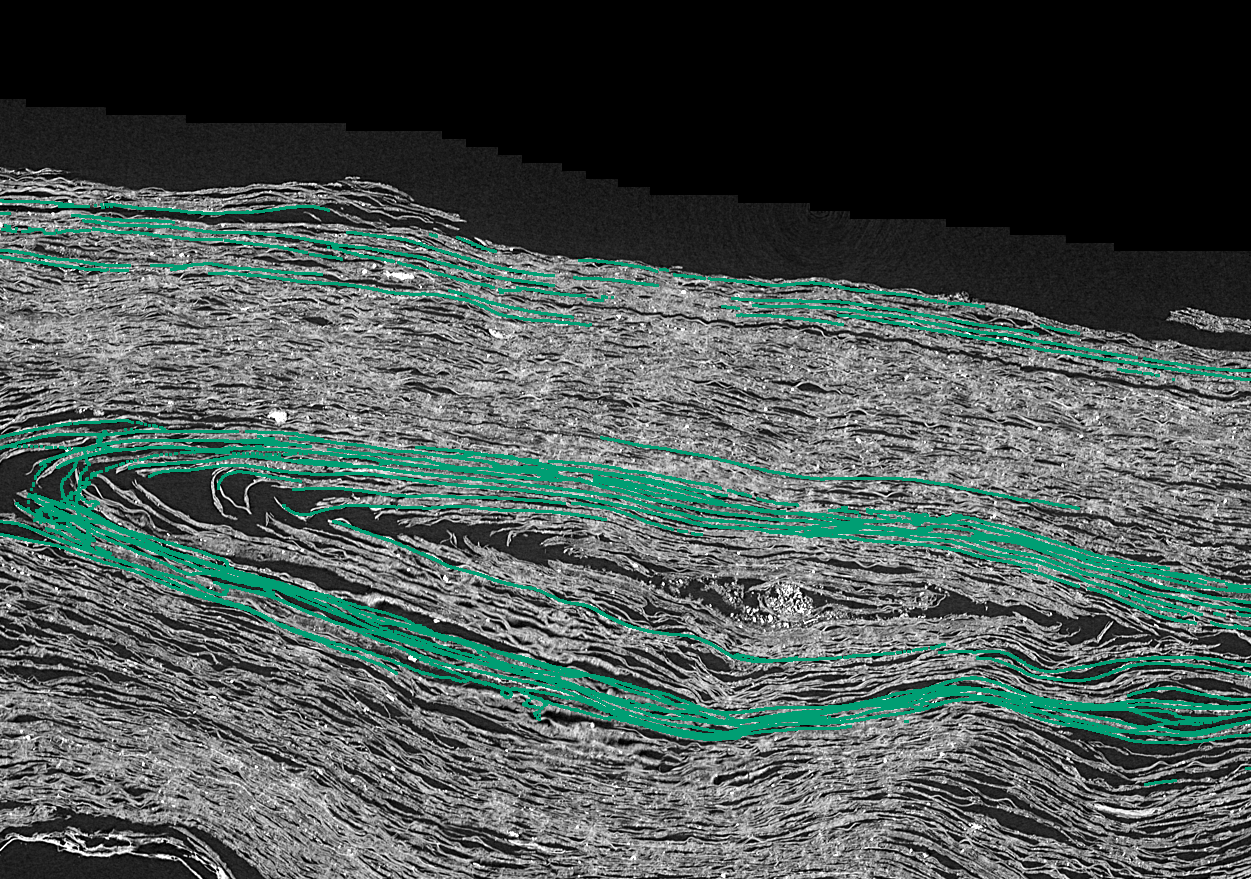
\includegraphics[width=8.6000cm]{../paper/figures/assets/c-f17-where-squares-slice-zoom.png}};
\node[hf] (m0) at (6.311,-4.704) {};
\node[hf] (m1) at (6.562,-4.819) {};
\node[hf] (m2) at (6.989,-3.341) {};
\node[hf] (m3) at (6.518,-4.777) {};
\node[hf] (m4) at (4.579,-4.716) {};
\node[ct] (m5) at (6.370,-4.939) {};
\node[ct] (m6) at (7.493,-3.499) {};
\node[ct] (m7) at (1.104,-1.103) {};
\node[lg] (m8) at (6.159,-4.598) {};
\node[lab, anchor=north west] (l2604) at (6.685,-4.106) {seed 2604\\\hfkey{} 17.7995 mm\\\lgkey{} 21.7474 mm};
\draw[lead] (m0) -- (l2604);
\draw[lead] (m8) -- (l2604);
\node[lab, anchor=north west] (l5364) at (4.616,-3.399) {seed 5364\\\hfkey{} 17.1642 mm\\\ctkey{} 15.3693 mm};
\draw[lead] (m1) -- (l5364);
\draw[lead] (m5) -- (l5364);
\node[lab, anchor=north west] (l1727) at (5.226,-2.105) {seed 1727\\\hfkey{} 17.0473 mm\\\ctkey{} 12.8975 mm};
\draw[lead] (m2) -- (l1727);
\draw[lead] (m6) -- (l1727);
\node[lab, anchor=north west] (l6273) at (4.503,-5.002) {seed 6273\\\hfkey{} 15.6438 mm};
\draw[lead] (m3) -- (l6273);
\node[lab, anchor=north west] (l4440) at (2.729,-3.567) {seed 4440\\\hfkey{} 15.1859 mm};
\draw[lead] (m4) -- (l4440);
\node[lab, anchor=north west] (l4480) at (1.554,-0.723) {seed 4480\\\ctkey{} 11.9670 mm};
\draw[lead] (m7) -- (l4480);
\node[note, anchor=south west] at (0.08,-5.963) {raw scan, no ink detector};
\node[key, anchor=north west] at (5.470,-0.080) {\sheetkey{} sheets of these seeds\\\ctkey{} certified square\\\hfkey{} hole free square\\\lgkey{} hole free, longer growth};

\end{tikzpicture}
\end{document}
